% Generated by Sphinx.
\def\sphinxdocclass{report}
\documentclass[letterpaper,10pt,english]{sphinxmanual}
\usepackage[utf8]{inputenc}
\DeclareUnicodeCharacter{00A0}{\nobreakspace}
\usepackage{cmap}
\usepackage[T1]{fontenc}
\usepackage{babel}
\usepackage{times}
\usepackage[Bjarne]{fncychap}
\usepackage{longtable}
\usepackage{sphinx}
\usepackage{multirow}

\addto\captionsenglish{\renewcommand{\figurename}{Fig. }}
\addto\captionsenglish{\renewcommand{\tablename}{Table }}
\floatname{literal-block}{Listing }



\title{Social Media Mining For Wheater Data Documentation}
\date{December 17, 2015}
\release{0.1}
\author{Dominic Looser}
\newcommand{\sphinxlogo}{}
\renewcommand{\releasename}{Release}
\makeindex

\makeatletter
\def\PYG@reset{\let\PYG@it=\relax \let\PYG@bf=\relax%
    \let\PYG@ul=\relax \let\PYG@tc=\relax%
    \let\PYG@bc=\relax \let\PYG@ff=\relax}
\def\PYG@tok#1{\csname PYG@tok@#1\endcsname}
\def\PYG@toks#1+{\ifx\relax#1\empty\else%
    \PYG@tok{#1}\expandafter\PYG@toks\fi}
\def\PYG@do#1{\PYG@bc{\PYG@tc{\PYG@ul{%
    \PYG@it{\PYG@bf{\PYG@ff{#1}}}}}}}
\def\PYG#1#2{\PYG@reset\PYG@toks#1+\relax+\PYG@do{#2}}

\expandafter\def\csname PYG@tok@vc\endcsname{\def\PYG@tc##1{\textcolor[rgb]{0.73,0.38,0.84}{##1}}}
\expandafter\def\csname PYG@tok@nn\endcsname{\let\PYG@bf=\textbf\def\PYG@tc##1{\textcolor[rgb]{0.05,0.52,0.71}{##1}}}
\expandafter\def\csname PYG@tok@sb\endcsname{\def\PYG@tc##1{\textcolor[rgb]{0.25,0.44,0.63}{##1}}}
\expandafter\def\csname PYG@tok@nt\endcsname{\let\PYG@bf=\textbf\def\PYG@tc##1{\textcolor[rgb]{0.02,0.16,0.45}{##1}}}
\expandafter\def\csname PYG@tok@s2\endcsname{\def\PYG@tc##1{\textcolor[rgb]{0.25,0.44,0.63}{##1}}}
\expandafter\def\csname PYG@tok@no\endcsname{\def\PYG@tc##1{\textcolor[rgb]{0.38,0.68,0.84}{##1}}}
\expandafter\def\csname PYG@tok@nc\endcsname{\let\PYG@bf=\textbf\def\PYG@tc##1{\textcolor[rgb]{0.05,0.52,0.71}{##1}}}
\expandafter\def\csname PYG@tok@c1\endcsname{\let\PYG@it=\textit\def\PYG@tc##1{\textcolor[rgb]{0.25,0.50,0.56}{##1}}}
\expandafter\def\csname PYG@tok@nd\endcsname{\let\PYG@bf=\textbf\def\PYG@tc##1{\textcolor[rgb]{0.33,0.33,0.33}{##1}}}
\expandafter\def\csname PYG@tok@mo\endcsname{\def\PYG@tc##1{\textcolor[rgb]{0.13,0.50,0.31}{##1}}}
\expandafter\def\csname PYG@tok@sx\endcsname{\def\PYG@tc##1{\textcolor[rgb]{0.78,0.36,0.04}{##1}}}
\expandafter\def\csname PYG@tok@gr\endcsname{\def\PYG@tc##1{\textcolor[rgb]{1.00,0.00,0.00}{##1}}}
\expandafter\def\csname PYG@tok@vg\endcsname{\def\PYG@tc##1{\textcolor[rgb]{0.73,0.38,0.84}{##1}}}
\expandafter\def\csname PYG@tok@m\endcsname{\def\PYG@tc##1{\textcolor[rgb]{0.13,0.50,0.31}{##1}}}
\expandafter\def\csname PYG@tok@na\endcsname{\def\PYG@tc##1{\textcolor[rgb]{0.25,0.44,0.63}{##1}}}
\expandafter\def\csname PYG@tok@sc\endcsname{\def\PYG@tc##1{\textcolor[rgb]{0.25,0.44,0.63}{##1}}}
\expandafter\def\csname PYG@tok@ge\endcsname{\let\PYG@it=\textit}
\expandafter\def\csname PYG@tok@gu\endcsname{\let\PYG@bf=\textbf\def\PYG@tc##1{\textcolor[rgb]{0.50,0.00,0.50}{##1}}}
\expandafter\def\csname PYG@tok@c\endcsname{\let\PYG@it=\textit\def\PYG@tc##1{\textcolor[rgb]{0.25,0.50,0.56}{##1}}}
\expandafter\def\csname PYG@tok@cs\endcsname{\def\PYG@tc##1{\textcolor[rgb]{0.25,0.50,0.56}{##1}}\def\PYG@bc##1{\setlength{\fboxsep}{0pt}\colorbox[rgb]{1.00,0.94,0.94}{\strut ##1}}}
\expandafter\def\csname PYG@tok@sd\endcsname{\let\PYG@it=\textit\def\PYG@tc##1{\textcolor[rgb]{0.25,0.44,0.63}{##1}}}
\expandafter\def\csname PYG@tok@il\endcsname{\def\PYG@tc##1{\textcolor[rgb]{0.13,0.50,0.31}{##1}}}
\expandafter\def\csname PYG@tok@kc\endcsname{\let\PYG@bf=\textbf\def\PYG@tc##1{\textcolor[rgb]{0.00,0.44,0.13}{##1}}}
\expandafter\def\csname PYG@tok@kd\endcsname{\let\PYG@bf=\textbf\def\PYG@tc##1{\textcolor[rgb]{0.00,0.44,0.13}{##1}}}
\expandafter\def\csname PYG@tok@ow\endcsname{\let\PYG@bf=\textbf\def\PYG@tc##1{\textcolor[rgb]{0.00,0.44,0.13}{##1}}}
\expandafter\def\csname PYG@tok@nv\endcsname{\def\PYG@tc##1{\textcolor[rgb]{0.73,0.38,0.84}{##1}}}
\expandafter\def\csname PYG@tok@kt\endcsname{\def\PYG@tc##1{\textcolor[rgb]{0.56,0.13,0.00}{##1}}}
\expandafter\def\csname PYG@tok@s\endcsname{\def\PYG@tc##1{\textcolor[rgb]{0.25,0.44,0.63}{##1}}}
\expandafter\def\csname PYG@tok@gs\endcsname{\let\PYG@bf=\textbf}
\expandafter\def\csname PYG@tok@nb\endcsname{\def\PYG@tc##1{\textcolor[rgb]{0.00,0.44,0.13}{##1}}}
\expandafter\def\csname PYG@tok@mi\endcsname{\def\PYG@tc##1{\textcolor[rgb]{0.13,0.50,0.31}{##1}}}
\expandafter\def\csname PYG@tok@gp\endcsname{\let\PYG@bf=\textbf\def\PYG@tc##1{\textcolor[rgb]{0.78,0.36,0.04}{##1}}}
\expandafter\def\csname PYG@tok@gi\endcsname{\def\PYG@tc##1{\textcolor[rgb]{0.00,0.63,0.00}{##1}}}
\expandafter\def\csname PYG@tok@mh\endcsname{\def\PYG@tc##1{\textcolor[rgb]{0.13,0.50,0.31}{##1}}}
\expandafter\def\csname PYG@tok@nf\endcsname{\def\PYG@tc##1{\textcolor[rgb]{0.02,0.16,0.49}{##1}}}
\expandafter\def\csname PYG@tok@ni\endcsname{\let\PYG@bf=\textbf\def\PYG@tc##1{\textcolor[rgb]{0.84,0.33,0.22}{##1}}}
\expandafter\def\csname PYG@tok@cp\endcsname{\def\PYG@tc##1{\textcolor[rgb]{0.00,0.44,0.13}{##1}}}
\expandafter\def\csname PYG@tok@gd\endcsname{\def\PYG@tc##1{\textcolor[rgb]{0.63,0.00,0.00}{##1}}}
\expandafter\def\csname PYG@tok@vi\endcsname{\def\PYG@tc##1{\textcolor[rgb]{0.73,0.38,0.84}{##1}}}
\expandafter\def\csname PYG@tok@ne\endcsname{\def\PYG@tc##1{\textcolor[rgb]{0.00,0.44,0.13}{##1}}}
\expandafter\def\csname PYG@tok@kp\endcsname{\def\PYG@tc##1{\textcolor[rgb]{0.00,0.44,0.13}{##1}}}
\expandafter\def\csname PYG@tok@mf\endcsname{\def\PYG@tc##1{\textcolor[rgb]{0.13,0.50,0.31}{##1}}}
\expandafter\def\csname PYG@tok@sh\endcsname{\def\PYG@tc##1{\textcolor[rgb]{0.25,0.44,0.63}{##1}}}
\expandafter\def\csname PYG@tok@k\endcsname{\let\PYG@bf=\textbf\def\PYG@tc##1{\textcolor[rgb]{0.00,0.44,0.13}{##1}}}
\expandafter\def\csname PYG@tok@se\endcsname{\let\PYG@bf=\textbf\def\PYG@tc##1{\textcolor[rgb]{0.25,0.44,0.63}{##1}}}
\expandafter\def\csname PYG@tok@s1\endcsname{\def\PYG@tc##1{\textcolor[rgb]{0.25,0.44,0.63}{##1}}}
\expandafter\def\csname PYG@tok@gt\endcsname{\def\PYG@tc##1{\textcolor[rgb]{0.00,0.27,0.87}{##1}}}
\expandafter\def\csname PYG@tok@si\endcsname{\let\PYG@it=\textit\def\PYG@tc##1{\textcolor[rgb]{0.44,0.63,0.82}{##1}}}
\expandafter\def\csname PYG@tok@ss\endcsname{\def\PYG@tc##1{\textcolor[rgb]{0.32,0.47,0.09}{##1}}}
\expandafter\def\csname PYG@tok@o\endcsname{\def\PYG@tc##1{\textcolor[rgb]{0.40,0.40,0.40}{##1}}}
\expandafter\def\csname PYG@tok@gh\endcsname{\let\PYG@bf=\textbf\def\PYG@tc##1{\textcolor[rgb]{0.00,0.00,0.50}{##1}}}
\expandafter\def\csname PYG@tok@go\endcsname{\def\PYG@tc##1{\textcolor[rgb]{0.20,0.20,0.20}{##1}}}
\expandafter\def\csname PYG@tok@cm\endcsname{\let\PYG@it=\textit\def\PYG@tc##1{\textcolor[rgb]{0.25,0.50,0.56}{##1}}}
\expandafter\def\csname PYG@tok@w\endcsname{\def\PYG@tc##1{\textcolor[rgb]{0.73,0.73,0.73}{##1}}}
\expandafter\def\csname PYG@tok@nl\endcsname{\let\PYG@bf=\textbf\def\PYG@tc##1{\textcolor[rgb]{0.00,0.13,0.44}{##1}}}
\expandafter\def\csname PYG@tok@bp\endcsname{\def\PYG@tc##1{\textcolor[rgb]{0.00,0.44,0.13}{##1}}}
\expandafter\def\csname PYG@tok@mb\endcsname{\def\PYG@tc##1{\textcolor[rgb]{0.13,0.50,0.31}{##1}}}
\expandafter\def\csname PYG@tok@err\endcsname{\def\PYG@bc##1{\setlength{\fboxsep}{0pt}\fcolorbox[rgb]{1.00,0.00,0.00}{1,1,1}{\strut ##1}}}
\expandafter\def\csname PYG@tok@sr\endcsname{\def\PYG@tc##1{\textcolor[rgb]{0.14,0.33,0.53}{##1}}}
\expandafter\def\csname PYG@tok@kn\endcsname{\let\PYG@bf=\textbf\def\PYG@tc##1{\textcolor[rgb]{0.00,0.44,0.13}{##1}}}
\expandafter\def\csname PYG@tok@kr\endcsname{\let\PYG@bf=\textbf\def\PYG@tc##1{\textcolor[rgb]{0.00,0.44,0.13}{##1}}}

\def\PYGZbs{\char`\\}
\def\PYGZus{\char`\_}
\def\PYGZob{\char`\{}
\def\PYGZcb{\char`\}}
\def\PYGZca{\char`\^}
\def\PYGZam{\char`\&}
\def\PYGZlt{\char`\<}
\def\PYGZgt{\char`\>}
\def\PYGZsh{\char`\#}
\def\PYGZpc{\char`\%}
\def\PYGZdl{\char`\$}
\def\PYGZhy{\char`\-}
\def\PYGZsq{\char`\'}
\def\PYGZdq{\char`\"}
\def\PYGZti{\char`\~}
% for compatibility with earlier versions
\def\PYGZat{@}
\def\PYGZlb{[}
\def\PYGZrb{]}
\makeatother

\renewcommand\PYGZsq{\textquotesingle}

\begin{document}

\maketitle
\tableofcontents
\phantomsection\label{index::doc}


Contents:


\chapter{Flickr}
\label{main/flickr:social-media-mining-for-wheater-data}\label{main/flickr:flickr}\label{main/flickr::doc}\begin{itemize}
\item {} 
Created by Ludicorp in 2004

\item {} 
Acquired by Yahoo in 2005

\item {} 
6 billion images in 2011 (we)

\item {} 
87 million registred users in 2013 (we)

\item {} 
3.5 million new images daily in 2013 (we)

\item {} 
Written in PHP

\end{itemize}


\section{API}
\label{main/flickr:api}\begin{itemize}
\item {} 
REST endpoint: \href{https://api.flickr.com/services/rest/}{https://api.flickr.com/services/rest/}

\item {} 
Return formats: XML, JSON, ...

\item {} 
Parameters: method, api\_key, format

\end{itemize}


\subsection{flickr.photos.search}
\label{main/flickr:flickr-photos-search}
Parameters:
\begin{itemize}
\item {} 
woe\_id: A 32-bit identifier that uniquely represents spatial entities

\item {} 
place\_id: A Flickr place id

\end{itemize}

Response structure:

\begin{DUlineblock}{0em}
\item[] photos \textgreater{} photo
\end{DUlineblock}

\begin{DUlineblock}{0em}
\item[] photos: page, pages, perpage, total
\item[] photo: id, latitude, longitude, place\_id, title, woeid
\end{DUlineblock}


\subsection{flickr.places.getInfo}
\label{main/flickr:flickr-places-getinfo}
Get informations about a place.
Parameters:
\begin{itemize}
\item {} 
woe\_id

\item {} 
place\_id

\end{itemize}

response structure:

\begin{DUlineblock}{0em}
\item[] rsp \textgreater{} place
\item[] place \textgreater{} country
\item[] country \textgreater{} shapedata
\item[] shapedate \textgreater{} polylines, urls
\item[] polylines \textgreater{} polyline
\item[] urls \textgreater{} shapefile
\end{DUlineblock}

\begin{DUlineblock}{0em}
\item[] rsp: stat
\item[] place: place\_id, woeid, latitutude, longitude, place\_url, place\_type, place\_type\_id, timezone, name, woe\_name, has\_shapedata
\item[] country: place\_id, woeid, latitutde, longitude, place\_url
\item[] shapedata: created, alpha, count\_points, count\_edges, has\_donuthole, is\_donuthole
\end{DUlineblock}


\subsection{flickr.places.find}
\label{main/flickr:flickr-places-find}
Returns a list of place objects for a given query string.

Parameter: query

Response:
\textbar{} rsp \textgreater{} places
\textbar{} places \textgreater{} place*

\begin{DUlineblock}{0em}
\item[] rsp: stat
\item[] places: query, total
\item[] place: place\_id, woeid, latitude, longitude, place\_url, place\_type
\end{DUlineblock}


\subsection{woe id vs place id}
\label{main/flickr:woe-id-vs-place-id}
WOE = where on earth


\section{Python Library}
\label{main/flickr:python-library}
We use the library called flickrapi. Documentation: \href{http://stuvel.eu/media/flickrapi-docs/documentation/}{http://stuvel.eu/media/flickrapi-docs/documentation/}


\chapter{Twitter}
\label{main/twitter::doc}\label{main/twitter:twitter}

\section{Basics}
\label{main/twitter:basics}\begin{itemize}
\item {} 
140 Characters per tweet

\item {} 
1.9 million tweets January 2009 (twitter api: up and running, p.4)

\item {} 
340 milion tweets each day (2012)

\item {} 
launched July 2006

\item {} 
Twitter Inc in San Francisco

\end{itemize}


\section{API}
\label{main/twitter:api}
Schema Tweet:

\begin{Verbatim}[commandchars=\\\{\}]
id
lang
text
created\PYGZus{}at
coordinates
   [coordinates]
place
entities
   [hashtags]
      text
   [urls]
\end{Verbatim}

Schema Place:

\begin{Verbatim}[commandchars=\\\{\}]
bounding\PYGZus{}box
   [coordinates]
      [float]
   type
contained\PYGZus{}within
country
country\PYGZus{}code
full\PYGZus{}name
name
place\PYGZus{}type
geometry
\end{Verbatim}


\subsection{REST-api}
\label{main/twitter:rest-api}
\href{https://api.twitter.com}{https://api.twitter.com}/\{version\}


\subsection{Search}
\label{main/twitter:search}
The Search API is not complete index of all Tweets, but instead an index of recent Tweets.
At the moment that index includes between 6-9 days of Tweets. (\href{https://dev.twitter.com/rest/public/search}{https://dev.twitter.com/rest/public/search})


\section{Tweepy}
\label{main/twitter:tweepy}
Python library used to connect to Twitter API through python.
\begin{description}
\item[{Schema Place}] \leavevmode
full\_name

\item[{Schema Status streaming-api:}] \leavevmode
contributors
truncated
text
in\_reply\_to\_status\_id
id
favorite\_count
author
\begin{quote}

User
follow\_request\_sent
profile\_use\_background\_image
\end{quote}
\begin{description}
\item[{\_json}] \leavevmode
follow\_request\_sent
profile\_use\_background\_image
default\_profile\_image
id
verified
profile\_image\_url\_https
profile\_sidebar\_fill\_color

\end{description}

\end{description}


\subsection{API}
\label{main/twitter:id1}\begin{itemize}
\item {} 
API.rate\_limit\_status (\href{http://docs.tweepy.org/en/v3.2.0/api.html\#API.rate\_limit\_status}{http://docs.tweepy.org/en/v3.2.0/api.html\#API.rate\_limit\_status})

\end{itemize}

Response Schema:

\begin{Verbatim}[commandchars=\\\{\}]
\PYGZob{}
    rate\PYGZus{}limit\PYGZus{}context
        access\PYGZus{}token
    resources
        *resource\PYGZus{}type*
            *resource\PYGZus{}name*
                limit
                remaining
                reset
\PYGZcb{}
\end{Verbatim}


\subsubsection{Geolocation}
\label{main/twitter:geolocation}\begin{itemize}
\item {} 
tweet is geotagged by user

\item {} 
in germany 1\% of tweets are geotagged

\item {} 
Approximately 3-5\% of all tweets are geo-enabled (\href{https://github.com/Ccantey/GeoSearch-Tweepy}{https://github.com/Ccantey/GeoSearch-Tweepy})

\item {} 
induce location from user profile

\item {} 
induce location from tweet text

\end{itemize}


\chapter{Helper APIs}
\label{main/helper-apis::doc}\label{main/helper-apis:helper-apis}

\section{World Weather Online}
\label{main/helper-apis:world-weather-online}

\subsection{Historical Weather API}
\label{main/helper-apis:historical-weather-api}
\href{http://www.worldweatheronline.com/api/docs/historical-weather-api.aspx}{docs}

response format:

\begin{Verbatim}[commandchars=\\\{\}]
data
    request
        type
        query
    [weather]
        date
        [hourly]
            precipMM
\end{Verbatim}


\chapter{Results}
\label{main/results::doc}\label{main/results:results}
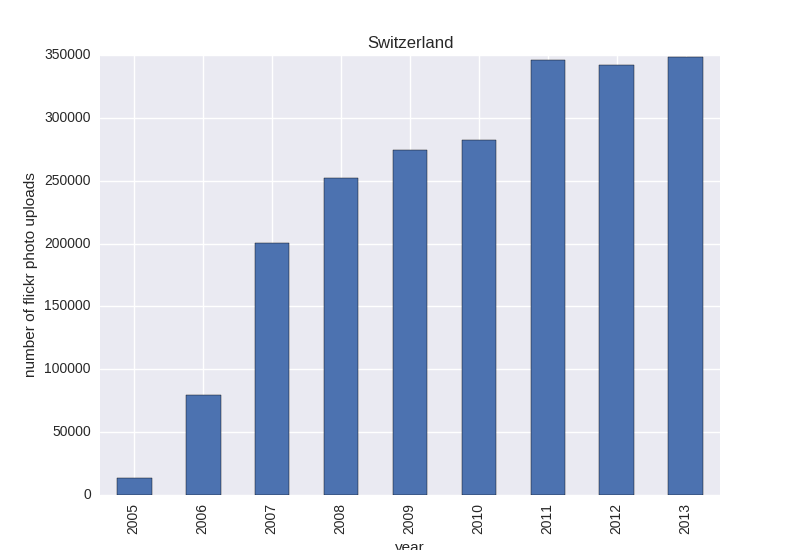
\includegraphics{flickr_switzerland.png}

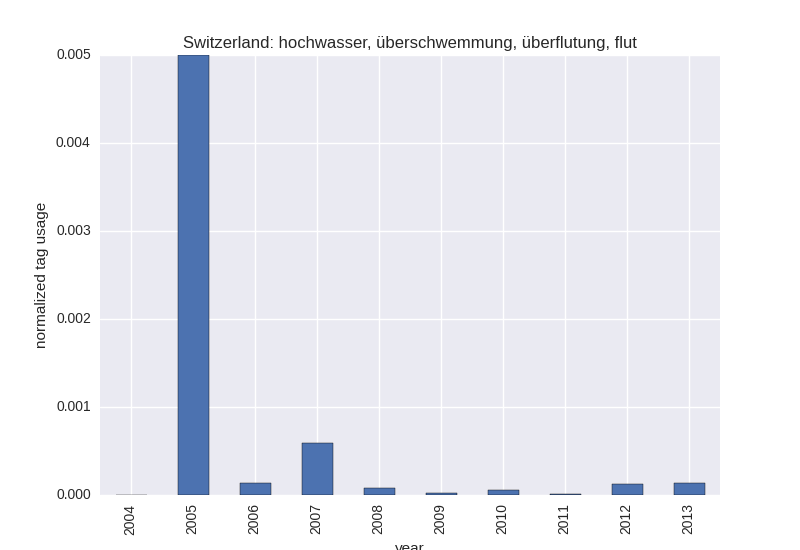
\includegraphics{flickr_flooding_switzerland.png}

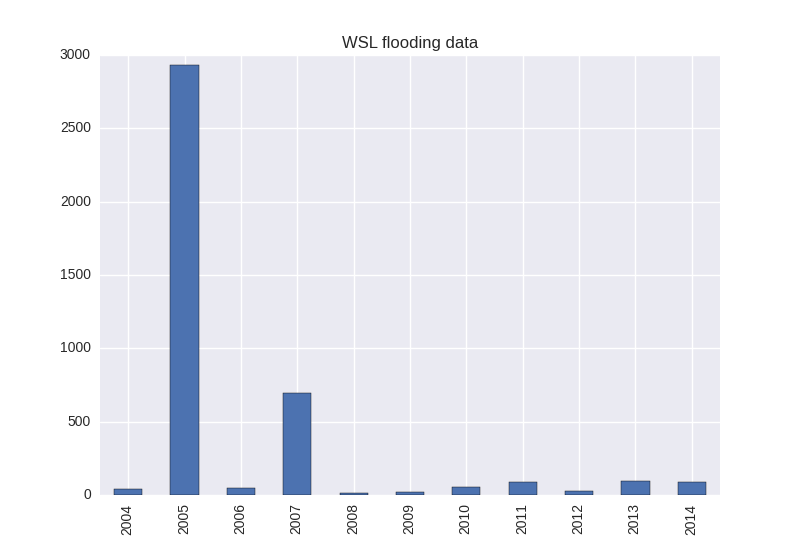
\includegraphics{wsl.png}


\chapter{Code}
\label{main/code::doc}\label{main/code:code}
All code is based on Python 3


\section{Install}
\label{main/code:install}\begin{itemize}
\item {} 
Install anaconda (\href{https://www.continuum.io/downloads}{https://www.continuum.io/downloads})

\item {} 
make a new conda environment called social-media-mining with:

\begin{Verbatim}[commandchars=\\\{\}]
conda env create \PYGZhy{}f .conda\PYGZus{}requirements.yml
\end{Verbatim}

\item {} 
activate this new environment with:

\begin{Verbatim}[commandchars=\\\{\}]
\PYG{n+nb}{source }activate social\PYGZhy{}media\PYGZhy{}mining
\end{Verbatim}

\item {} 
download source code from git ...

\item {} 
create new file called local\_config.py in folder main with the line
\begin{quote}

ROOT\_DIR = path to you the root folder of the project
\end{quote}

\end{itemize}


\section{Important Libraries}
\label{main/code:important-libraries}\begin{itemize}
\item {} 
Pandas (data analysis)

\item {} 
Matplotlib/Seaborn (plotting)

\item {} 
flickrapi

\item {} 
tweepy

\item {} 
nltk (natural language processing)

\end{itemize}


\chapter{.}
\label{modules::doc}\label{modules:id1}

\section{main package}
\label{main::doc}\label{main:main-package}

\subsection{Submodules}
\label{main:submodules}

\subsection{main.flickr\_analysis module}
\label{main:main-flickr-analysis-module}

\subsection{main.geo module}
\label{main:main-geo-module}\label{main:module-main.geo}\index{main.geo (module)}\index{BoundingBox (class in main.geo)}

\begin{fulllineitems}
\phantomsection\label{main:main.geo.BoundingBox}\pysiglinewithargsret{\strong{class }\code{main.geo.}\bfcode{BoundingBox}}{\emph{twitter\_bounding\_box=None}}{}
Bases: \code{object}

\end{fulllineitems}

\index{Map (class in main.geo)}

\begin{fulllineitems}
\phantomsection\label{main:main.geo.Map}\pysiglinewithargsret{\strong{class }\code{main.geo.}\bfcode{Map}}{\emph{bounding\_box}, \emph{map\_resolution=\textless{}MapResolution.INTERMEDIATE: 1\textgreater{}}}{}
Bases: \code{object}
\index{draw\_densities() (main.geo.Map method)}

\begin{fulllineitems}
\phantomsection\label{main:main.geo.Map.draw_densities}\pysiglinewithargsret{\bfcode{draw\_densities}}{\emph{points}, \emph{n\_bins}, \emph{color\_map='Blues'}}{}
\end{fulllineitems}

\index{draw\_points() (main.geo.Map method)}

\begin{fulllineitems}
\phantomsection\label{main:main.geo.Map.draw_points}\pysiglinewithargsret{\bfcode{draw\_points}}{\emph{points}}{}
\end{fulllineitems}

\index{save() (main.geo.Map method)}

\begin{fulllineitems}
\phantomsection\label{main:main.geo.Map.save}\pysiglinewithargsret{\bfcode{save}}{\emph{path}, \emph{format='png'}}{}
\end{fulllineitems}

\index{show() (main.geo.Map method)}

\begin{fulllineitems}
\phantomsection\label{main:main.geo.Map.show}\pysiglinewithargsret{\bfcode{show}}{}{}
\end{fulllineitems}


\end{fulllineitems}

\index{MapResolution (class in main.geo)}

\begin{fulllineitems}
\phantomsection\label{main:main.geo.MapResolution}\pysigline{\strong{class }\code{main.geo.}\bfcode{MapResolution}}
Bases: \code{enum.Enum}

An enumeration.
\index{FULL (main.geo.MapResolution attribute)}

\begin{fulllineitems}
\phantomsection\label{main:main.geo.MapResolution.FULL}\pysigline{\bfcode{FULL}\strong{ = \textless{}MapResolution.FULL: 2\textgreater{}}}
\end{fulllineitems}

\index{INTERMEDIATE (main.geo.MapResolution attribute)}

\begin{fulllineitems}
\phantomsection\label{main:main.geo.MapResolution.INTERMEDIATE}\pysigline{\bfcode{INTERMEDIATE}\strong{ = \textless{}MapResolution.INTERMEDIATE: 1\textgreater{}}}
\end{fulllineitems}


\end{fulllineitems}

\index{Place (class in main.geo)}

\begin{fulllineitems}
\phantomsection\label{main:main.geo.Place}\pysiglinewithargsret{\strong{class }\code{main.geo.}\bfcode{Place}}{\emph{twitter\_place}, \emph{wunderground\_id: str}}{}
Bases: \code{object}

\end{fulllineitems}

\index{Point (class in main.geo)}

\begin{fulllineitems}
\phantomsection\label{main:main.geo.Point}\pysigline{\strong{class }\code{main.geo.}\bfcode{Point}}
Bases: \code{object}

\end{fulllineitems}

\index{draw\_map() (in module main.geo)}

\begin{fulllineitems}
\phantomsection\label{main:main.geo.draw_map}\pysiglinewithargsret{\code{main.geo.}\bfcode{draw\_map}}{\emph{place}}{}
\end{fulllineitems}



\subsection{main.local\_config module}
\label{main:main-local-config-module}\label{main:module-main.local_config}\index{main.local\_config (module)}

\subsection{main.store module}
\label{main:main-store-module}

\subsection{main.twitter\_analysis module}
\label{main:main-twitter-analysis-module}

\subsection{main.utils module}
\label{main:main-utils-module}\label{main:module-main.utils}\index{main.utils (module)}\index{Stopwatch (class in main.utils)}

\begin{fulllineitems}
\phantomsection\label{main:main.utils.Stopwatch}\pysigline{\strong{class }\code{main.utils.}\bfcode{Stopwatch}}
Bases: \code{object}
\index{start() (main.utils.Stopwatch method)}

\begin{fulllineitems}
\phantomsection\label{main:main.utils.Stopwatch.start}\pysiglinewithargsret{\bfcode{start}}{}{}
\end{fulllineitems}


\end{fulllineitems}

\index{save\_plot() (in module main.utils)}

\begin{fulllineitems}
\phantomsection\label{main:main.utils.save_plot}\pysiglinewithargsret{\code{main.utils.}\bfcode{save\_plot}}{\emph{plot\_id}, \emph{directory}}{}
\end{fulllineitems}



\subsection{Module contents}
\label{main:module-main}\label{main:module-contents}\index{main (module)}

\renewcommand{\indexname}{Python Module Index}
\begin{theindex}
\def\bigletter#1{{\Large\sffamily#1}\nopagebreak\vspace{1mm}}
\bigletter{m}
\item {\texttt{main}}, \pageref{main:module-main}
\item {\texttt{main.geo}}, \pageref{main:module-main.geo}
\item {\texttt{main.local\_config}}, \pageref{main:module-main.local_config}
\item {\texttt{main.utils}}, \pageref{main:module-main.utils}
\end{theindex}

\renewcommand{\indexname}{Index}
\printindex
\end{document}
